%!TeX root=../tese.tex
%("dica" para o editor de texto: este arquivo é parte de um documento maior)
% para saber mais: https://tex.stackexchange.com/q/78101/183146

%% ------------------------------------------------------------------------- %%
\chapter{Delimitações inferiores de Wilber}
\label{cap:wilber}

\newcommand{\cT}{\mathcal{T}}

Nesse capítulo buscaremos entender o comportamento do custo $OPT(X)$ para diferentes sequências de acesso $X$. Compreenderemos o funcionamento das delimitações propostas por Wilber \cite{lowerbound_wilber} e relacionaremos essas delimitações com a delimitação dos retângulos independentes do capítulo anterior.

\section{Visão geral}

Wilber foi o pioneiro na área de buscar delimitações inferiores de custo em algoritmos de busca em ABBs que permitem rotações. Durante sua pesquisa, Wilber desenvolveu duas delimitações que ficaram conhecidas como Wilber I e Wilber II. Posteriormente, essas delimitações foram denominadas, respectivamente, delimitação da alternância e delimitação do funil. 

Essas delimitações foram propostas se utilizando de nomenclatura, definições e provas bastante complicadas. Nesse trabalho, ao invés de mostrar tais provas, mostraremos que essas delimitações podem ser interpretadas como ferramentas para encontrar conjuntos de retângulos independentes. Assim, ficará evidente que a delimitação de retângulos independentes é pelo menos tão boa quanto ambas as delimitações propostas por Wilber.

Inicialmente, será necessário definir uma série de conceitos que serão usados posteriormente.
Dados dois conjuntos $L$ e $R$ finitos e disjuntos de pontos. Denotaremos por $mix(L,R)$ a string em $\{$\textbf{L},\textbf{R}$\}^{*}$ obtida pela união $L \cup R$ em ordem crescente, substituindo cada elemento de $L$ por \textbf{L} e cada elemento de $R$ por \textbf{R}. Para os conjuntos $L = \{2,3,6\}$ e $R = \{1,4,5\}$, $mix(L,R)$ = \textbf{RLLRRL}. Essa string final é uma representação das posições relativas dos pontos em ordem crescente.

Dada uma string $s \in \{$\textbf{L},\textbf{R}$\}^{*}$, definimos $blocos(s)$ como o número de blocos contíguos do mesmo símbolo em $s$. Assim,

\[
blocos(s) = 
\begin{cases}
    0, & \text{se s é vazia}. \\
    1 + \#\{i \mid s_i \neq s_{i+1}\}, & \text{caso contrário}.
\end{cases}
\]

Por exemplo, blocos(\textbf{RLLRRL}) = 4.

Para finalizar, definimos $intercala(L,R) = blocos(mix(L,R))$. Assim, compactamos as definições acima para produzir a função $intercala$ que recebe dois conjuntos de pontos e retornar um inteiro que representa o número de blocos contíguos do mesmo símbolo da string resultante de $mix(L,R)$. Assim, para o exemplo acima $intercala(L,R) = 4$.

%precisa falar que os conjuntos possuem y-coordenadas distintas?

\section{Delimitação da Alternância}

Seja $P$ um conjunto de pontos. Uma \textit{árvore de referência} $\cT$ em relação à $P$ é uma árvore binária em que todo nó não-folha possui dois filhos e as folhas são rotuladas com os valores de $P$\hspace{-0.05cm}$.x$ em ordem crescente. Veja a Figura~\ref{fig:arvore_de_referencia_exemplo_inicial}. Note que para conjuntos de pontos com $|P| > 2$, há múltiplas árvores de referência em relação à $P$.
\begin{figure}
    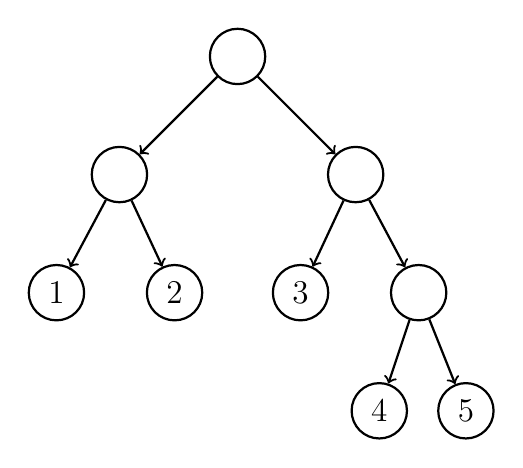
\begin{tikzpicture}
        [node/.style={circle,draw,minimum size=2em, thick, font=\large},
        nodeGray/.style={circle,draw,minimum size=2em, thick, font=\large, fill=gray!55}]
        \node[node] (D) at (0,0) {};
        \node[node] (B) at (-1.5,-1.5) {};
        \node[node] (A) at (-2.3,-3) {$1$};
        \node[node] (C) at (-0.8,-3) {$2$};
        \node[node] (E) at (0.8,-3) {$3$};
        \node[node] (F) at (1.5,-1.5) {};
        \node[node] (G) at (2.3,-3) {};
        \node[node] (H) at (1.8,-4.5) {$4$};
        \node[node] (I) at (2.9,-4.5) {$5$};
        
        \draw[thick, ->] (D) -- (B);%node[midway, left, yshift=0.15cm, xshift=0.08cm] {\textbf{E}};
        \draw[thick, ->] (B) -- (A);%node[midway, left, yshift=0.15cm, xshift=0.08cm] {\textbf{E}};
        \draw[thick, ->] (B) -- (C);%node[midway, right, yshift=0.15cm, xshift=-0.08cm] {\textbf{D}};
        \draw[thick, ->] (G) -- (I);%node[midway, right, yshift=0.15cm, xshift=-0.08cm] {\textbf{D}};
        \draw[thick, ->] (G) -- (H);%node[midway, left, yshift=0.15cm, xshift=0.08cm] {\textbf{E}};
        
        \draw[thick, ->] (D) -- (F);%node[midway, right, yshift=0.15cm, xshift=-0.08cm] {\textbf{D}};
        \draw[thick, ->] (F) -- (E);%node[midway, left, yshift=0.15cm, xshift=0.08cm] {\textbf{E}};
        \draw[thick, ->] (F) -- (G);%node[midway, right, yshift=0.15cm, xshift=-0.08cm] {\textbf{D}};
    
    \end{tikzpicture}
    \caption{Uma árvore de referência $\cT$ para o conjunto de pontos de $P_X$ da sequência de acessos $X = (3,1,4,2,5)$.}
\label{fig:arvore_de_referencia_exemplo_inicial}
\end{figure}

Definimos Alt$_{\cT}$ de maneira recursiva. Se $\cT$ for um nó único, então Alt$_{\cT} = 0$. Caso contrário, seja $\cT_{L}$ e $\cT_{R}$ respectivamente a subárvore esquerda e a subárvore direita da raiz de $\cT$. Denotamos por $P_L = \{p \in P \mid p.x \in \cT_L\}$ e $P_R = \{p \in P \mid p.x \in \cT_R\}$. 

Definimos $a(P,\cT) = intercala(P_L.y, P_R.y)$, que mostra como se intercalaram os pontos em $P_L$ e $P_R$ de maneira cronológica. Por fim, definimos a delimitação da alternância para um conjunto de pontos $P$ em relação à árvore de referência $\cT$ como:

Alt$_\cT(P) = a(P,\cT) +$ Alt$_{\cT_L}(P_L) + $ Alt$_{\cT_R}(P_R)$.

Note que a delimitação da alternância de um conjunto de pontos $P$ pode ter valores diferentes dependendo da escolha da árvore de referência. Veja a Figura~\ref{fig:alternancia_diferente}. Assim, definimos a delimitação da alternância para uma sequência de acessos $X$ como o valor da maior delimitação da alternância para a visão geométrica de $X$ em relação à uma árvore de referência. Formalmente: 

Alt$(X) = max_\cT$ Alt$_\cT(P_X)$.

\begin{comment}
    \begin{figure}
        \begin{minipage}[b]{0.45\textwidth}
            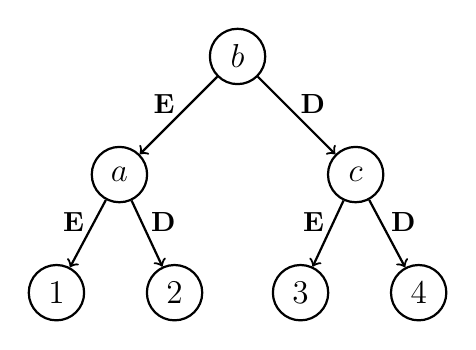
\begin{tikzpicture}
                [node/.style={circle,draw,minimum size=2em, thick, font=\large},
        nodeGray/.style={circle,draw,minimum size=2em, thick, font=\large, fill=gray!55}]
                \node[node] (D) at (0,0) {$b$};
                \node[node] (B) at (-1.5,-1.5) {$a$};
                \node[node] (A) at (-2.3,-3) {$1$};
                \node[node] (C) at (-0.8,-3) {$2$};
                \node[node] (E) at (0.8,-3) {$3$};
                \node[node] (F) at (1.5,-1.5) {$c$};
                \node[node] (G) at (2.3,-3) {$4$};
                
                \draw[thick, ->] (D) -- (B) node[midway, left, yshift=0.15cm, xshift=0.08cm] {\textbf{E}};
                \draw[thick, ->] (B) -- (A) node[midway, left, yshift=0.15cm, xshift=0.08cm] {\textbf{E}};
                \draw[thick, ->] (B) -- (C) node[midway, right, yshift=0.15cm, xshift=-0.08cm] {\textbf{D}};
                
                \draw[thick, ->] (D) -- (F) node[midway, right, yshift=0.15cm, xshift=-0.08cm] {\textbf{D}};
                \draw[thick, ->] (F) -- (E) node[midway, left, yshift=0.15cm, xshift=0.08cm] {\textbf{E}};
                \draw[thick, ->] (F) -- (G) node[midway, right, yshift=0.15cm, xshift=-0.08cm] {\textbf{D}};
            \end{tikzpicture}
        \end{minipage} \hfill
        \begin{minipage}[b]{0.45\textwidth}
            \vfill
            \begin{tabular}{>{\centering\arraybackslash}p{0.7cm} >{\centering\arraybackslash}p{5cm} p{0.3cm}} % Define as larguras das colunas
                Nó & Alternância de filhos & \# \\
                \hline
                a & D, E, D  & 3 \\
                b & D, E, E, D, E, D  & 5  \\
                c & E, D, E  & 3  \\
                \hline
                Total  &   & 11  \\
            \end{tabular}
            \vfill
        \end{minipage}
        \caption{3,2,1,4,2,3}
    \end{figure}
\end{comment}

\begin{figure}
    \begin{minipage}[c]{0.3\textwidth} % Alinhar ao centro
        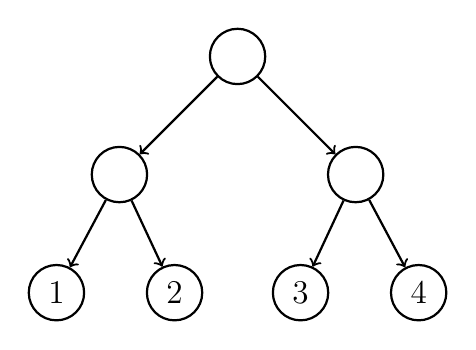
\begin{tikzpicture}
            [node/.style={circle,draw,minimum size=2em, thick, font=\large},
        nodeGray/.style={circle,draw,minimum size=2em, thick, font=\large, fill=gray!55}]
            \node[node] (D) at (0,0) {};
            \node[node] (B) at (-1.5,-1.5) {};
            \node[node] (A) at (-2.3,-3) {$1$};
            \node[node] (C) at (-0.8,-3) {$2$};
            \node[node] (E) at (0.8,-3) {$3$};
            \node[node] (F) at (1.5,-1.5) {};
            \node[node] (G) at (2.3,-3) {$4$};
            
            \draw[thick, ->] (D) -- (B); % node[midway, left, yshift=0.15cm, xshift=0.08cm] {\textbf{E}};
            \draw[thick, ->] (B) -- (A); % node[midway, left, yshift=0.15cm, xshift=0.08cm] {\textbf{E}};
            \draw[thick, ->] (B) -- (C); % node[midway, right, yshift=0.15cm, xshift=-0.08cm] {\textbf{D}};
            
            \draw[thick, ->] (D) -- (F); % node[midway, right, yshift=0.15cm, xshift=-0.08cm] {\textbf{D}};
            \draw[thick, ->] (F) -- (E); % node[midway, left, yshift=0.15cm, xshift=0.08cm] {\textbf{E}};
            \draw[thick, ->] (F) -- (G); % node[midway, right, yshift=0.15cm, xshift=-0.08cm] {\textbf{D}};
        \end{tikzpicture}
    \end{minipage} \hfill
    \begin{minipage}[c]{0.59\textwidth} % Alinhar ao centro
        \vfill % Preenche o espaço vertical
        \begin{tabular}{>{\centering\arraybackslash}p{1.4cm} >{\centering\arraybackslash}p{5cm} >{\centering\arraybackslash}p{1.5cm}} % Define as larguras das colunas
            Alt & $blocos(mix(E,D))$ & $intercala$ \\
            \hline
            Alt$_\cT(P)$ & [D], [E,E], [D], [E], [D]  & 5 \\
            Alt$_{\cT_E}(P_E)$ & [D], [E], [D]  & 3  \\
            Alt$_{\cT_D}(P_D)$ & [E], [D], [E]  & 3  \\
            \hline
            Total  &   & 11  \\
        \end{tabular}
        \vfill % Preenche o espaço vertical
    \end{minipage}
    \caption{Alt$_\cT(P_X)$ calculada para a árvore de referência $\cT$ acima e para a sequência de acessos $X = (3,2,1,4,2,3)$.}
\end{figure}

\begin{figure}
    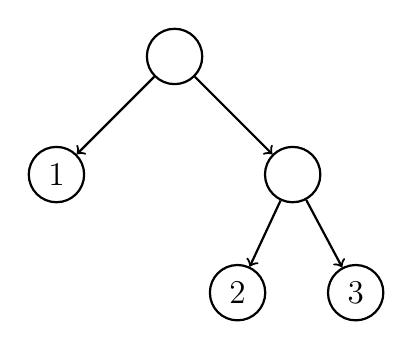
\begin{tikzpicture}
        [node/.style={circle,draw,minimum size=2em, thick, font=\large},
        nodeGray/.style={circle,draw,minimum size=2em, thick, font=\large, fill=gray!55}]
        \node[node] (D) at (0,0) {};
        \node[node] (B) at (-1.5,-1.5) {$1$};
        \node[node] (E) at (0.8,-3) {$2$};
        \node[node] (F) at (1.5,-1.5) {};
        \node[node] (G) at (2.3,-3) {$3$};
        
        \draw[thick, ->] (D) -- (B); % node[midway, left, yshift=0.15cm, xshift=0.08cm] {\textbf{E}};
        
        \draw[thick, ->] (D) -- (F); % node[midway, right, yshift=0.15cm, xshift=-0.08cm] {\textbf{D}};
        \draw[thick, ->] (F) -- (E); % node[midway, left, yshift=0.15cm, xshift=0.08cm] {\textbf{E}};
        \draw[thick, ->] (F) -- (G); % node[midway, right, yshift=0.15cm, xshift=-0.08cm] {\textbf{D}};
    \end{tikzpicture}
    \hspace{1cm}
    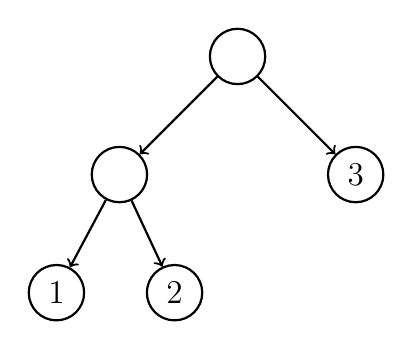
\begin{tikzpicture}
        [node/.style={circle,draw,minimum size=2em, thick, font=\large},
        nodeGray/.style={circle,draw,minimum size=2em, thick, font=\large, fill=gray!55}]
        \node[node] (D) at (0,0) {};
        \node[node] (B) at (-1.5,-1.5) {};
        \node[node] (A) at (-2.3,-3) {$1$};
        \node[node] (C) at (-0.8,-3) {$2$};
        \node[node] (F) at (1.5,-1.5) {$3$};
        
        \draw[thick, ->] (D) -- (B); % node[midway, left, yshift=0.15cm, xshift=0.08cm] {\textbf{E}};
        \draw[thick, ->] (B) -- (A); % node[midway, left, yshift=0.15cm, xshift=0.08cm] {\textbf{E}};
        \draw[thick, ->] (B) -- (C); % node[midway, right, yshift=0.15cm, xshift=-0.08cm] {\textbf{D}};
        
        \draw[thick, ->] (D) -- (F); % node[midway, right, yshift=0.15cm, xshift=-0.08cm] {\textbf{D}};
    \end{tikzpicture}
    \caption{À esquerda $\cT_1$ e à direita $\cT_2$. Perceba que para a sequência de buscas $X = (1,3,2)$, Alt$_{\cT_1}(P_X) = 4$, enquanto que Alt$_{\cT_2}(P_X) = 5$.}
\label{fig:alternancia_diferente}
\end{figure}

%Alt$_{\cT_L}(P_L)

Para contribuir com a intuição do leitor, a seguir mostraremos uma maneira alternativa e bem mais informal de entender essa delimitação. Apesar de árvores de referência não serem árvores binárias de busca, uma vez que os nós não possuem atributo chave, é possível contabilizar essa delimitação simulando buscas pelos rótulos das folhas nessa árvore. Para todo nó não-folha de $\cT$, definimos como \textit{filho preferido} deste nó o filho mais recentemente visitado, podendo ser o filho esquerdo, o filho direito ou, se nenhum dos dois filhos tiver sido visitado ainda, o valor nulo.

Assim, dado um sequência de acessos $X$ e uma árvore de referência $\cT$ em relação à $P_X$, se simularmos as buscas de $X$ em $\cT$, ou seja, simular um algoritmo de busca que sempre inicializa na raiz de $\cT$ e para cada busca o algoritmo visita apenas os nós intermediários de $\cT$ que estão no caminho da raiz de $\cT$ a folha com rótulo buscado. Essa árvore é fixa, ou seja, o algoritmo de busca não pode realizar rotações. Veja a Figura~\ref{fig:alternancia_abordagem_informal}.

Assim, Alt$_\cT(X)$ é o somatório do número de vezes que o filho preferido de cada nó intermediário foi alterado. Analogamente, Alt$(X) = max_\cT$ Alt$_\cT(X)$. Então, Alt$(X)$ é o somatório do número de vezes que o filho preferido de cada nó intermediário foi alterado em uma árvore de referência que maximiza esse número.

Infelizmente essa delimitação não é justa se permitirmos repetições na sequência $X$ de acessos. Uma maneira facil de perceber que $OPT(X)$ pode ser muito maior que Alt$(X)$ é observando como a delimitação se comporta quando $X$ possui repetições do mesmo acesso consecutivamente. Quando simulamos a mesma busca em sequência em uma árvore de referência nenhum filho preferido é alterado, então a delimitação não aumenta.

Sabemos que todo acesso tem custo maior ou igual a 1 e assim $OPT(X) \geq m$, mas devido a essas repetições, é possível que $m$ seja arbitrariamente maior que Alt$(X)$. Para entender o argumento acima, se atente às últimas duas simulações de busca na Figura~\ref{fig:alternancia_abordagem_informal}.

\begin{figure}[H]
    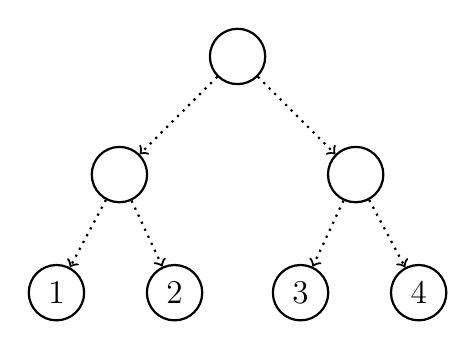
\begin{tikzpicture}
        [node/.style={circle,draw,minimum size=2em, thick, font=\large},
        nodeGray/.style={circle,draw,minimum size=2em, thick, font=\large, fill=gray!55}]
        \node[node] (D) at (0,0) {};
        \node[node] (B) at (-1.5,-1.5) {};
        \node[node] (A) at (-2.3,-3) {$1$};
        \node[node] (C) at (-0.8,-3) {$2$};
        \node[node] (E) at (0.8,-3) {$3$};
        \node[node] (F) at (1.5,-1.5) {};
        \node[node] (G) at (2.3,-3) {$4$};
        
        \draw[thick, dotted, ->] (D) -- (B);%node[midway, left, yshift=0.15cm, xshift=0.08cm] {\textbf{E}};
        \draw[thick, dotted, ->] (B) -- (A);%node[midway, left, yshift=0.15cm, xshift=0.08cm] {\textbf{E}};
        \draw[thick, dotted, ->] (B) -- (C);%node[midway, right, yshift=0.15cm, xshift=-0.08cm] {\textbf{D}};
        
        \draw[thick, dotted, ->] (D) -- (F);%node[midway, right, yshift=0.15cm, xshift=-0.08cm] {\textbf{D}};
        \draw[thick, dotted, ->] (F) -- (E);%node[midway, left, yshift=0.15cm, xshift=0.08cm] {\textbf{E}};
        \draw[thick, dotted, ->] (F) -- (G);%node[midway, right, yshift=0.15cm, xshift=-0.08cm] {\textbf{D}};
    
    \end{tikzpicture}
    \hspace{1cm}
    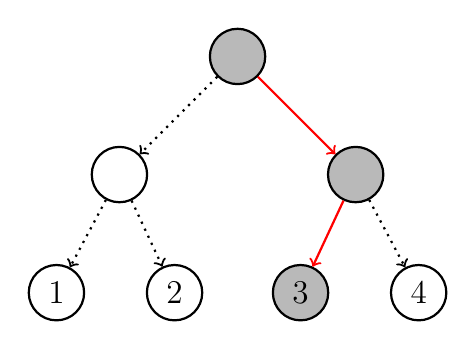
\begin{tikzpicture}
        [node/.style={circle,draw,minimum size=2em, thick, font=\large},
        nodeGray/.style={circle,draw,minimum size=2em, thick, font=\large, fill=gray!55}]
        \node[nodeGray] (D) at (0,0) {};
        \node[node] (B) at (-1.5,-1.5) {};
        \node[node] (A) at (-2.3,-3) {$1$};
        \node[node] (C) at (-0.8,-3) {$2$};
        \node[nodeGray] (E) at (0.8,-3) {$3$};
        \node[nodeGray] (F) at (1.5,-1.5) {};
        \node[node] (G) at (2.3,-3) {$4$};
        
        \draw[thick, dotted, ->] (D) -- (B);%node[midway, left, yshift=0.15cm, xshift=0.08cm] {\textbf{E}};
        \draw[thick, dotted, ->] (B) -- (A);%node[midway, left, yshift=0.15cm, xshift=0.08cm] {\textbf{E}};
        \draw[thick, dotted, ->] (B) -- (C);%node[midway, right, yshift=0.15cm, xshift=-0.08cm] {\textbf{D}};
        
        \draw[thick, ->, red] (D) -- (F);%node[midway, right, yshift=0.15cm, xshift=-0.08cm] {\textbf{D}};
        \draw[thick, ->, red] (F) -- (E);%node[midway, left, yshift=0.15cm, xshift=0.08cm] {\textbf{E}};
        \draw[thick, dotted, ->] (F) -- (G);%node[midway, right, yshift=0.15cm, xshift=-0.08cm] {\textbf{D}};
    
    \end{tikzpicture}
    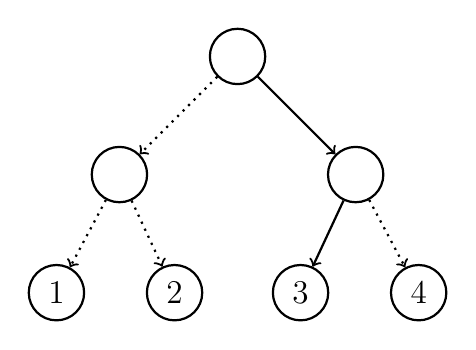
\begin{tikzpicture}
        [node/.style={circle,draw,minimum size=2em, thick, font=\large},
        nodeGray/.style={circle,draw,minimum size=2em, thick, font=\large, fill=gray!55}]
        \node[node] (D) at (0,0) {};
        \node[node] (B) at (-1.5,-1.5) {};
        \node[node] (A) at (-2.3,-3) {$1$};
        \node[node] (C) at (-0.8,-3) {$2$};
        \node[node] (E) at (0.8,-3) {$3$};
        \node[node] (F) at (1.5,-1.5) {};
        \node[node] (G) at (2.3,-3) {$4$};
        
        \draw[thick, dotted, ->] (D) -- (B);%node[midway, left, yshift=0.15cm, xshift=0.08cm] {\textbf{E}};
        \draw[thick, dotted, ->] (B) -- (A);%node[midway, left, yshift=0.15cm, xshift=0.08cm] {\textbf{E}};
        \draw[thick, dotted, ->] (B) -- (C);%node[midway, right, yshift=0.15cm, xshift=-0.08cm] {\textbf{D}};
        
        \draw[thick, ->] (D) -- (F);%node[midway, right, yshift=0.15cm, xshift=-0.08cm] {\textbf{D}};
        \draw[thick, ->] (F) -- (E);%node[midway, left, yshift=0.15cm, xshift=0.08cm] {\textbf{E}};
        \draw[thick, dotted, ->] (F) -- (G);%node[midway, right, yshift=0.15cm, xshift=-0.08cm] {\textbf{D}};
    
    \end{tikzpicture}
    \hspace{1cm}
    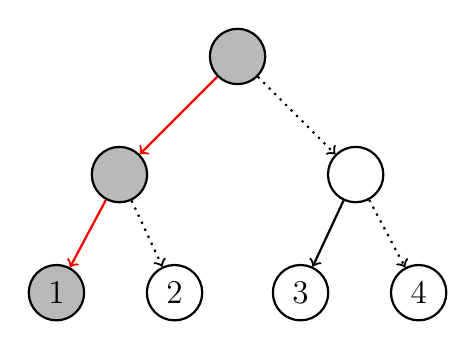
\begin{tikzpicture}
        [node/.style={circle,draw,minimum size=2em, thick, font=\large},
        nodeGray/.style={circle,draw,minimum size=2em, thick, font=\large, fill=gray!55}]
        \node[nodeGray] (D) at (0,0) {};
        \node[nodeGray] (B) at (-1.5,-1.5) {};
        \node[nodeGray] (A) at (-2.3,-3) {$1$};
        \node[node] (C) at (-0.8,-3) {$2$};
        \node[node] (E) at (0.8,-3) {$3$};
        \node[node] (F) at (1.5,-1.5) {};
        \node[node] (G) at (2.3,-3) {$4$};
        
        \draw[thick, ->, red] (D) -- (B);%node[midway, left, yshift=0.15cm, xshift=0.08cm] {\textbf{E}};
        \draw[thick, ->, red] (B) -- (A);%node[midway, left, yshift=0.15cm, xshift=0.08cm] {\textbf{E}};
        \draw[thick, dotted, ->] (B) -- (C);%node[midway, right, yshift=0.15cm, xshift=-0.08cm] {\textbf{D}};
        
        \draw[thick, dotted, ->] (D) -- (F);%node[midway, right, yshift=0.15cm, xshift=-0.08cm] {\textbf{D}};
        \draw[thick, ->] (F) -- (E);%node[midway, left, yshift=0.15cm, xshift=0.08cm] {\textbf{E}};
        \draw[thick, dotted, ->] (F) -- (G);%node[midway, right, yshift=0.15cm, xshift=-0.08cm] {\textbf{D}};
    
    \end{tikzpicture}
    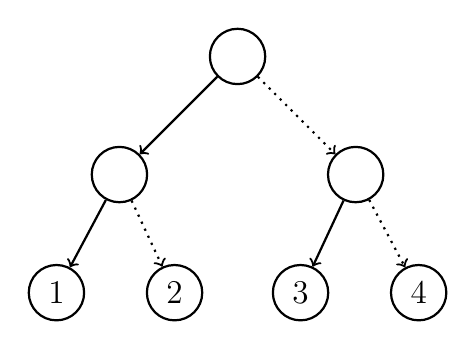
\begin{tikzpicture}
        [node/.style={circle,draw,minimum size=2em, thick, font=\large},
        nodeGray/.style={circle,draw,minimum size=2em, thick, font=\large, fill=gray!55}]
        \node[node] (D) at (0,0) {};
        \node[node] (B) at (-1.5,-1.5) {};
        \node[node] (A) at (-2.3,-3) {$1$};
        \node[node] (C) at (-0.8,-3) {$2$};
        \node[node] (E) at (0.8,-3) {$3$};
        \node[node] (F) at (1.5,-1.5) {};
        \node[node] (G) at (2.3,-3) {$4$};
        
        \draw[thick, ->] (D) -- (B);%node[midway, left, yshift=0.15cm, xshift=0.08cm] {\textbf{E}};
        \draw[thick, ->] (B) -- (A);%node[midway, left, yshift=0.15cm, xshift=0.08cm] {\textbf{E}};
        \draw[thick, dotted, ->] (B) -- (C);%node[midway, right, yshift=0.15cm, xshift=-0.08cm] {\textbf{D}};
        
        \draw[thick, dotted, ->] (D) -- (F);%node[midway, right, yshift=0.15cm, xshift=-0.08cm] {\textbf{D}};
        \draw[thick, ->] (F) -- (E);%node[midway, left, yshift=0.15cm, xshift=0.08cm] {\textbf{E}};
        \draw[thick, dotted, ->] (F) -- (G);%node[midway, right, yshift=0.15cm, xshift=-0.08cm] {\textbf{D}};
    
    \end{tikzpicture}
    \hspace{1cm}
    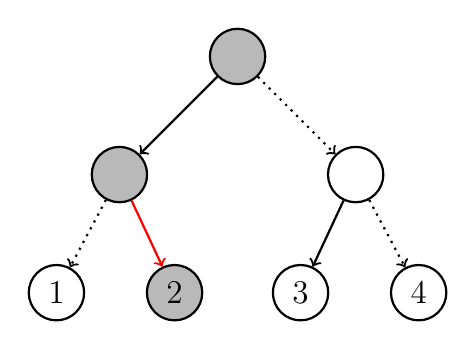
\begin{tikzpicture}
        [node/.style={circle,draw,minimum size=2em, thick, font=\large},
        nodeGray/.style={circle,draw,minimum size=2em, thick, font=\large, fill=gray!55}]
        \node[nodeGray] (D) at (0,0) {};
        \node[nodeGray] (B) at (-1.5,-1.5) {};
        \node[node] (A) at (-2.3,-3) {$1$};
        \node[nodeGray] (C) at (-0.8,-3) {$2$};
        \node[node] (E) at (0.8,-3) {$3$};
        \node[node] (F) at (1.5,-1.5) {};
        \node[node] (G) at (2.3,-3) {$4$};
        
        \draw[thick, ->] (D) -- (B);%node[midway, left, yshift=0.15cm, xshift=0.08cm] {\textbf{E}};
        \draw[thick, dotted, ->] (B) -- (A);%node[midway, left, yshift=0.15cm, xshift=0.08cm] {\textbf{E}};
        \draw[thick, ->, red] (B) -- (C);%node[midway, right, yshift=0.15cm, xshift=-0.08cm] {\textbf{D}};
        
        \draw[thick, dotted, ->] (D) -- (F);%node[midway, right, yshift=0.15cm, xshift=-0.08cm] {\textbf{D}};
        \draw[thick, ->] (F) -- (E);%node[midway, left, yshift=0.15cm, xshift=0.08cm] {\textbf{E}};
        \draw[thick, dotted, ->] (F) -- (G);%node[midway, right, yshift=0.15cm, xshift=-0.08cm] {\textbf{D}};
    
    \end{tikzpicture}
    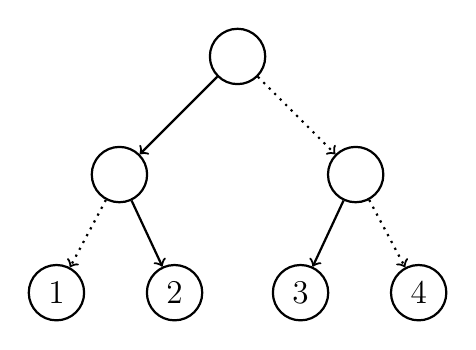
\begin{tikzpicture}
        [node/.style={circle,draw,minimum size=2em, thick, font=\large},
        nodeGray/.style={circle,draw,minimum size=2em, thick, font=\large, fill=gray!55}]
        \node[node] (D) at (0,0) {};
        \node[node] (B) at (-1.5,-1.5) {};
        \node[node] (A) at (-2.3,-3) {$1$};
        \node[node] (C) at (-0.8,-3) {$2$};
        \node[node] (E) at (0.8,-3) {$3$};
        \node[node] (F) at (1.5,-1.5) {};
        \node[node] (G) at (2.3,-3) {$4$};
        
        \draw[thick, ->] (D) -- (B);%node[midway, left, yshift=0.15cm, xshift=0.08cm] {\textbf{E}};
        \draw[thick, dotted, ->] (B) -- (A);%node[midway, left, yshift=0.15cm, xshift=0.08cm] {\textbf{E}};
        \draw[thick, ->] (B) -- (C);%node[midway, right, yshift=0.15cm, xshift=-0.08cm] {\textbf{D}};
        
        \draw[thick, dotted, ->] (D) -- (F);%node[midway, right, yshift=0.15cm, xshift=-0.08cm] {\textbf{D}};
        \draw[thick, ->] (F) -- (E);%node[midway, left, yshift=0.15cm, xshift=0.08cm] {\textbf{E}};
        \draw[thick, dotted, ->] (F) -- (G);%node[midway, right, yshift=0.15cm, xshift=-0.08cm] {\textbf{D}};
    
    \end{tikzpicture}
    \hspace{1cm}
    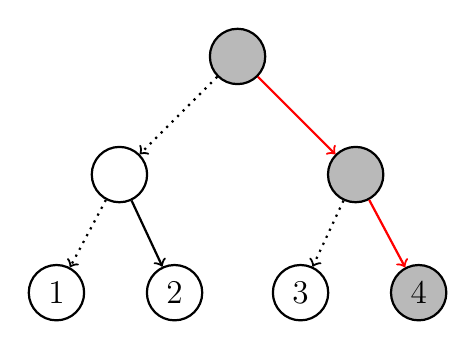
\begin{tikzpicture}
        [node/.style={circle,draw,minimum size=2em, thick, font=\large},
        nodeGray/.style={circle,draw,minimum size=2em, thick, font=\large, fill=gray!55}]
        \node[nodeGray] (D) at (0,0) {};
        \node[node] (B) at (-1.5,-1.5) {};
        \node[node] (A) at (-2.3,-3) {$1$};
        \node[node] (C) at (-0.8,-3) {$2$};
        \node[node] (E) at (0.8,-3) {$3$};
        \node[nodeGray] (F) at (1.5,-1.5) {};
        \node[nodeGray] (G) at (2.3,-3) {$4$};
        
        \draw[thick, dotted, ->] (D) -- (B);%node[midway, left, yshift=0.15cm, xshift=0.08cm] {\textbf{E}};
        \draw[thick, dotted, ->] (B) -- (A);%node[midway, left, yshift=0.15cm, xshift=0.08cm] {\textbf{E}};
        \draw[thick, ->] (B) -- (C);%node[midway, right, yshift=0.15cm, xshift=-0.08cm] {\textbf{D}};
        
        \draw[thick, ->, red] (D) -- (F);%node[midway, right, yshift=0.15cm, xshift=-0.08cm] {\textbf{D}};
        \draw[thick, dotted, ->] (F) -- (E);%node[midway, left, yshift=0.15cm, xshift=0.08cm] {\textbf{E}};
        \draw[thick, ->, red] (F) -- (G);%node[midway, right, yshift=0.15cm, xshift=-0.08cm] {\textbf{D}};
    \end{tikzpicture}
    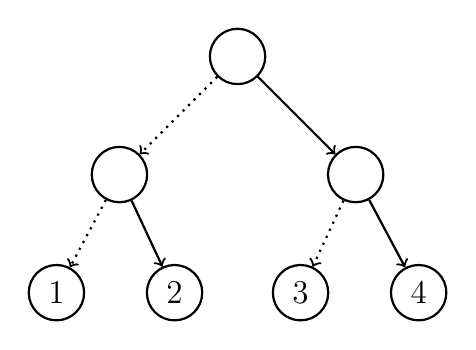
\begin{tikzpicture}
        [node/.style={circle,draw,minimum size=2em, thick, font=\large},
        nodeGray/.style={circle,draw,minimum size=2em, thick, font=\large, fill=gray!55}]
        \node[node] (D) at (0,0) {};
        \node[node] (B) at (-1.5,-1.5) {};
        \node[node] (A) at (-2.3,-3) {$1$};
        \node[node] (C) at (-0.8,-3) {$2$};
        \node[node] (E) at (0.8,-3) {$3$};
        \node[node] (F) at (1.5,-1.5) {};
        \node[node] (G) at (2.3,-3) {$4$};
        
        \draw[thick, dotted, ->] (D) -- (B);%node[midway, left, yshift=0.15cm, xshift=0.08cm] {\textbf{E}};
        \draw[thick, dotted, ->] (B) -- (A);%node[midway, left, yshift=0.15cm, xshift=0.08cm] {\textbf{E}};
        \draw[thick, ->] (B) -- (C);%node[midway, right, yshift=0.15cm, xshift=-0.08cm] {\textbf{D}};
        
        \draw[thick, ->] (D) -- (F);%node[midway, right, yshift=0.15cm, xshift=-0.08cm] {\textbf{D}};
        \draw[thick, dotted, ->] (F) -- (E);%node[midway, left, yshift=0.15cm, xshift=0.08cm] {\textbf{E}};
        \draw[thick, ->] (F) -- (G);%node[midway, right, yshift=0.15cm, xshift=-0.08cm] {\textbf{D}};
    \end{tikzpicture}
    \hspace{1cm}
    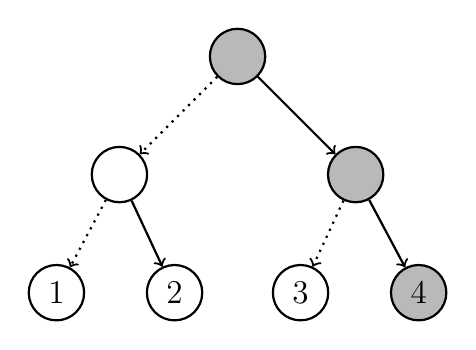
\begin{tikzpicture}
        [node/.style={circle,draw,minimum size=2em, thick, font=\large},
        nodeGray/.style={circle,draw,minimum size=2em, thick, font=\large, fill=gray!55}]
        \node[nodeGray] (D) at (0,0) {};
        \node[node] (B) at (-1.5,-1.5) {};
        \node[node] (A) at (-2.3,-3) {$1$};
        \node[node] (C) at (-0.8,-3) {$2$};
        \node[node] (E) at (0.8,-3) {$3$};
        \node[nodeGray] (F) at (1.5,-1.5) {};
        \node[nodeGray] (G) at (2.3,-3) {$4$};
        
        \draw[thick, dotted, ->] (D) -- (B);%node[midway, left, yshift=0.15cm, xshift=0.08cm] {\textbf{E}};
        \draw[thick, dotted, ->] (B) -- (A);%node[midway, left, yshift=0.15cm, xshift=0.08cm] {\textbf{E}};
        \draw[thick, ->] (B) -- (C);%node[midway, right, yshift=0.15cm, xshift=-0.08cm] {\textbf{D}};
        
        \draw[thick, ->] (D) -- (F);%node[midway, right, yshift=0.15cm, xshift=-0.08cm] {\textbf{D}};
        \draw[thick, dotted, ->] (F) -- (E);%node[midway, left, yshift=0.15cm, xshift=0.08cm] {\textbf{E}};
        \draw[thick, ->] (F) -- (G);%node[midway, right, yshift=0.15cm, xshift=-0.08cm] {\textbf{D}};
    \end{tikzpicture}
    
    \caption{Cálculo de Alt$_\cT(X)$ para a sequência de buscas $X = (3,1,2,4,4)$ e a árvore de referência $\cT$ ilustrada. À esquerda, as árvores antes da simulação de buscas. À direita, a simulação de cada busca. Os ponteiros que representam filhos preferidos estão por inteiro enquanto que os ponteiros que representam filhos não-preferidos estão pontilhados. Durante as simulações de busca, estão em vermelho os filhos preferidos que foram alterados durante aquela busca. Note que Alt$_\cT(X) = 7$, pois esse é o número de filhos preferidos alterados (ponteiros vermelhos) durante as buscas.}
\label{fig:alternancia_abordagem_informal}
\end{figure}

\section{Alternância em retângulos independentes}

Dada uma sequência $X$ de acessos e uma árvore de referência $\cT$ em relação à $P_X$, é possível encontrar os retângulos independentes relacionados à esta delimitação a partir do seguinte algoritmo: Inicialize o algoritmo verificando o nó raiz de $\cT$, seja $u$ o maior rótulo de um nó da subárvore esquerda da raiz e $v$ o menor rótulo de um nó da subárvore direita da raiz. Trace uma reta vertical na visão 2D de $P_X$ na coordenada $x = \frac{u + v}{2}$. Desenhe um retângulo para cada par de pontos consecutivos que possuem a propriedade que um dos pontos está a esquerda da reta traçada e o outro a direita. Assim, recursivamente analise o vértice filho esquerdo da raiz de $\cT$ porém considerando apenas os pontos à esquerda da reta traçada anteriormente e também analise o vértice filho direito da raiz de $\cT$ porém considerando apenas os pontos à direita da reta traçada.

O algoritmo recursivamente encontra pares de pontos. Esses pares de pontos têm a propriedade que um deles está à esquerda da linha vertical analisada e o outro à direita. Por serem pontos consecutivos com essa propriedade, então sabemos que não há nenhum outro ponto dentro da área deste par de pontos e por serem pontos diferentes

\section{Delimitação do Funil}

Seja $P$ um conjunto de pontos. Definimos o \textit{funil esquerdo} de um ponto $p$ de $P$ como o conjunto de pontos de $P$ que possuem as seguintes propriedades: estão à esquerda de $p$, abaixo de $p$ e o retângulo ortogonal que possui $p$ e algum ponto do funil esquerdo de $p$ como vértices não possui nenhum outro ponto de $P$. Formalmente, 

$F_E(P,p) = \{q \in P \mid q.y < p.y \; \land \; q.x < p.x \; \land \; \{p,q\}\text{-retângulo é arboreamente insatisfeito}\}$

De maneira simétrica definimos o \textit{funil direito},

$F_D(P,p) = \{q \in P \mid q.y > p.y \; \land \; q.x < p.x \; \land \; \{p,q\}\text{-retângulo é arboreamente insatisfeito}\}$

Por fim, definimos o \textit{funil} de $p$ como a união do funil esquerdo e do funil direito de $p$, ou seja, $F_E(P,p) \cup F_D(P,p)$.

\begin{comment}
    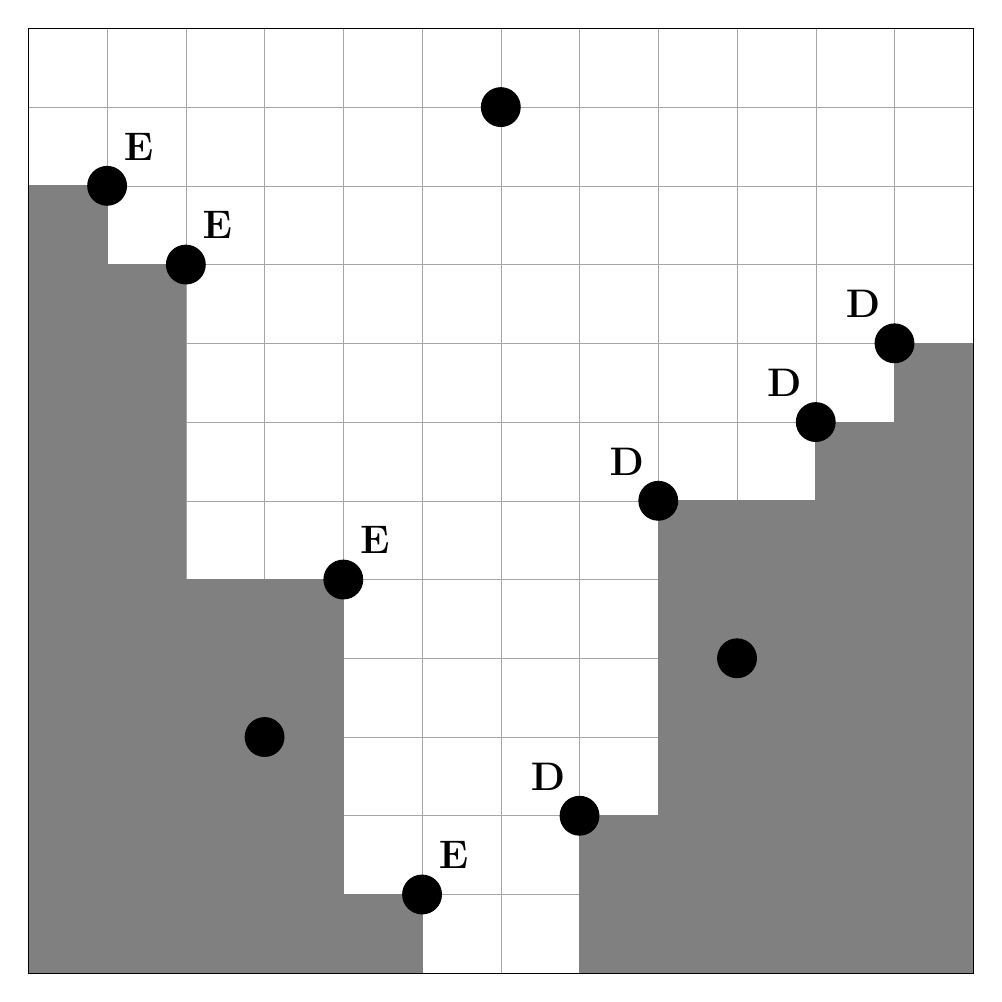
\begin{tikzpicture}[scale=1]
        \draw[very thin, gray!70] (0,0) grid (12,12);
        
        \draw[fill=gray, gray] (0,0) rectangle (1,10);
        \draw[fill=gray, gray] (1,0) rectangle (2,9);
        \draw[fill=gray, gray] (2,0) rectangle (4,5);
        \draw[fill=gray, gray] (4,0) rectangle (5,1);
        \draw[fill=gray, gray] (11,8) rectangle (12,0);
        \draw[fill=gray, gray] (10,7) rectangle (11,0);
        \draw[fill=gray, gray] (8,6) rectangle (10,0);
        \draw[fill=gray, gray] (7,2) rectangle (8,0);

        \filldraw[black] (5,1) circle (7pt);
        \filldraw[black] (7,2) circle (7pt);
        \filldraw[black] (3,3) circle (7pt);
        \filldraw[black] (9,4) circle (7pt);
        \filldraw[black] (4,5) circle (7pt);
        \filldraw[black] (8,6) circle (7pt);
        \filldraw[black] (10,7) circle (7pt);
        \filldraw[black] (11,8) circle (7pt);
        \filldraw[black] (2,9) circle (7pt);
        \filldraw[black] (1,10) circle (7pt);
        \filldraw[black] (6,11) circle (7pt);
        \node at (1.4,10.5) {\textbf{\Large E}};
        \node at (2.4,9.5) {\textbf{\Large E}};
        \node at (4.4,5.5) {\textbf{\Large E}};
        \node at (5.4,1.5) {\textbf{\Large E}};
        \node at (10.6,8.5) {\textbf{\Large D}};
        \node at (9.6,7.5) {\textbf{\Large D}};
        \node at (7.6,6.5) {\textbf{\Large D}};
        \node at (6.6,2.5) {\textbf{\Large D}};
        \draw[black, line width=0.5pt] (0,0) rectangle (12,12);
    \end{tikzpicture}
\end{comment}

\definecolor{color_of_analysed_point}{named}{blue}

\begin{figure}
    \centering
    \begin{tikzpicture}[scale=0.62]
        \draw[very thin, gray!70] (0,0) grid (8,8);

        \draw[color_of_analysed_point, dashed, line width=1.5pt] (4,0) -- (4,8);
        
        %\draw[red, line width=1.2pt] (1,5) rectangle (4,7);
        %\draw[red, line width=1.2pt] (3,3) rectangle (4,7);
        
        \filldraw[black] (2,1) circle (7pt);
        \filldraw[red] (3,3) circle (7pt);
        \filldraw[black] (5,2) circle (7pt);
        \filldraw[black] (7,4) circle (7pt);
        \filldraw[red] (1,5) circle (7pt);
        \filldraw[black] (6,6) circle (7pt);
        \filldraw[color_of_analysed_point] (4,7) circle (7pt);
        \draw[black, line width=0.5pt] (0,0) rectangle (8,8);
    \end{tikzpicture}
    \begin{tikzpicture}[scale=0.62]
        \draw[very thin, gray!70] (0,0) grid (8,8);
        \draw[color_of_analysed_point, dashed, line width=1.5pt] (4,0) -- (4,8);
        
        %\draw[red, line width=1.2pt] (5,2) rectangle (4,7);
        %\draw[red, line width=1.2pt] (6,6) rectangle (4,7);
        
        \filldraw[black] (2,1) circle (7pt);
        \filldraw[black] (3,3) circle (7pt);
        \filldraw[red] (5,2) circle (7pt);
        \filldraw[black] (7,4) circle (7pt);
        \filldraw[black] (1,5) circle (7pt);
        \filldraw[red] (6,6) circle (7pt);
        \filldraw[color_of_analysed_point] (4,7) circle (7pt);
        \draw[black, line width=0.5pt] (0,0) rectangle (8,8);
    \end{tikzpicture}
    \begin{tikzpicture}[scale=0.62]
        \draw[very thin, gray!70] (0,0) grid (8,8);
        %\draw[color_of_analysed_point, dashed, line width=1.5pt] (4,0) -- (4,8);
        
        \filldraw[black] (2,1) circle (7pt);
        \filldraw[red] (3,3) circle (7pt);
        \filldraw[red] (5,2) circle (7pt);
        \filldraw[black] (7,4) circle (7pt);
        \filldraw[red] (1,5) circle (7pt);
        \filldraw[red] (6,6) circle (7pt);
        \filldraw[color_of_analysed_point] (4,7) circle (7pt);
        \draw[black, line width=0.5pt] (0,0) rectangle (8,8);
    \end{tikzpicture}
    %\caption{Nesta visão geométrica de uma sequência de acessos, está destacado de azul o ponto (4,7). À esquerda, estão destacados de vermelho os pontos do Funil esquerdo do ponto azul. Ao meio, estão destacados os pontos do Funil direito do ponto azul. À direita, estão destacados os pontos pertencentes ao funil do ponto azul.}
    \caption{O ponto (4,7) está destacado. À esquerda, os pontos vermelhos pertencem ao funil esquerdo do ponto azul. Ao meio, os pontos vermelhos pertencem ao funil direito do ponto azul. À direita, estão destacados de vermelho os pontos do funil do ponto azul, que são a união dos dois conjuntos anteriores.}
\end{figure}

A delimitação do funil para um ponto conta o número de alternâncias entre o funil esquerdo e o funil direito desse ponto, assim para cada ponto $p$ de $P$, definimos $f(P,p) = intercala(F_L(P,p).y, F_R(P,p).y)$. A delimitação do funil para uma sequência $X$ de acessos é a somatória desse valor para todos os pontos da visão geométrica de $X$, ou seja, Funil$(X) = \sum_{p \in P_X}^{f(P_X,p)}$.

De maneira informal, a ideia central dessa delimitação é somar o valor de $f(P_X,p)$ para cada ponto $p \in P_X$. Assim, para cada ponto de $P_X$, calcule o número de intercalações direita-esquerda dos pontos abaixo dele, indo de cima para baixo, cujas x-coordenadas se aproximam da x-coordenada do ponto analisado.

\begin{comment}
\begin{figure}
    \centering
    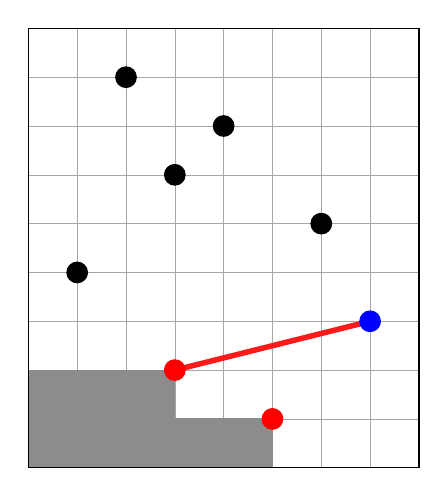
\begin{tikzpicture}[scale=0.62]
        \draw[very thin, gray!70] (0,0) grid (8,9);
        
        \draw[fill=gray!90, gray!90] (0,0) rectangle (3,2);
        \draw[fill=gray!90, gray!90] (1,0) rectangle (5,1);

        \draw[red!90, line width=2pt] (7,3) -- (3,2);  

        \filldraw[red] (5,1) circle (6pt);
        \filldraw[red] (3,2) circle (6pt);
        \filldraw[blue] (7,3) circle (6pt);
        \filldraw[black] (1,4) circle (6pt);
        \filldraw[black] (6,5) circle (6pt);
        \filldraw[black] (3,6) circle (6pt);
        \filldraw[black] (4,7) circle (6pt);
        \filldraw[black] (2,8) circle (6pt);


        %\node at (1,9.5) {\textbf{\Large E}};
        %\node at (2,8.5) {\textbf{\Large E}};
        %\node at (4,5.5) {\textbf{\Large E}};
        %\node at (5,1.5) {\textbf{\Large E}};

        %\node at (10,7.5) {\textbf{\Large D}};
        %\node at (8,6.5) {\textbf{\Large D}};
        %\node at (7,2.5) {\textbf{\Large D}};


        \draw[black, line width=0.5pt] (0,0) rectangle (8,9);
    \end{tikzpicture}
    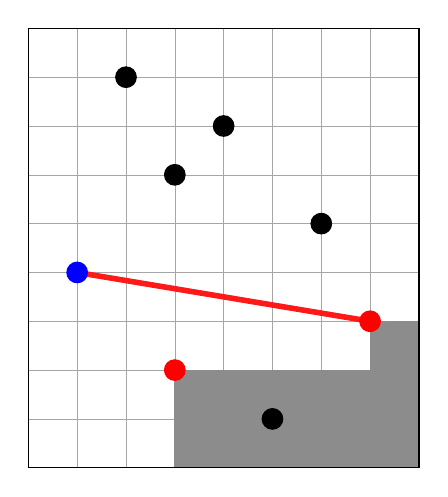
\begin{tikzpicture}[scale=0.62]
        \draw[very thin, gray!70] (0,0) grid (8,9);
        
        \draw[fill=gray!90, gray!90] (8,0) rectangle (3,2);
        \draw[fill=gray!90, gray!90] (8,0) rectangle (7,3);

        \draw[red!90, line width=2pt] (1,4) -- (7,3); 

        \filldraw[black] (5,1) circle (6pt);
        \filldraw[red] (3,2) circle (6pt);
        \filldraw[red] (7,3) circle (6pt);
        \filldraw[blue] (1,4) circle (6pt);
        \filldraw[black] (6,5) circle (6pt);
        \filldraw[black] (3,6) circle (6pt);
        \filldraw[black] (4,7) circle (6pt);
        \filldraw[black] (2,8) circle (6pt);


        %\node at (1,9.5) {\textbf{\Large E}};
        %\node at (2,8.5) {\textbf{\Large E}};
        %\node at (4,5.5) {\textbf{\Large E}};
        %\node at (5,1.5) {\textbf{\Large E}};

        %\node at (10,7.5) {\textbf{\Large D}};
        %\node at (8,6.5) {\textbf{\Large D}};
        %\node at (7,2.5) {\textbf{\Large D}};


        \draw[black, line width=0.5pt] (0,0) rectangle (8,9);
    \end{tikzpicture}
    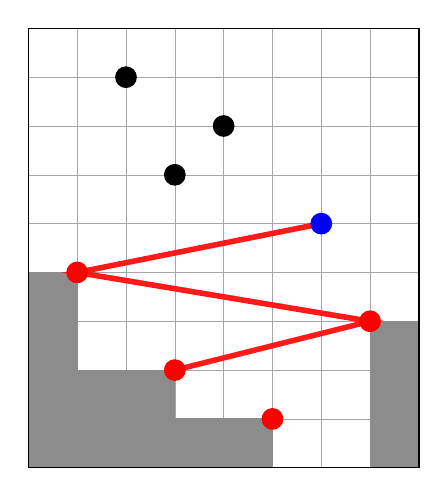
\begin{tikzpicture}[scale=0.62] %3
        \draw[very thin, gray!70] (0,0) grid (8,9);
        
        \draw[fill=gray!90, gray!90] (0,0) rectangle (5,1);
        \draw[fill=gray!90, gray!90] (0,0) rectangle (3,2);
        \draw[fill=gray!90, gray!90] (8,0) rectangle (7,3);
        \draw[fill=gray!90, gray!90] (0,0) rectangle (1,4);

        \draw[red!90, line width=2pt] (6,5) -- (1,4) -- (7,3) -- (3,2);

        \filldraw[red] (5,1) circle (6pt);
        \filldraw[red] (3,2) circle (6pt);
        \filldraw[red] (7,3) circle (6pt);
        \filldraw[red] (1,4) circle (6pt);
        \filldraw[blue] (6,5) circle (6pt);
        \filldraw[black] (3,6) circle (6pt);
        \filldraw[black] (4,7) circle (6pt);
        \filldraw[black] (2,8) circle (6pt);


        %\node at (1,9.5) {\textbf{\Large E}};
        %\node at (2,8.5) {\textbf{\Large E}};
        %\node at (4,5.5) {\textbf{\Large E}};
        %\node at (5,1.5) {\textbf{\Large E}};

        %\node at (10,7.5) {\textbf{\Large D}};
        %\node at (8,6.5) {\textbf{\Large D}};
        %\node at (7,2.5) {\textbf{\Large D}};


        \draw[black, line width=0.5pt] (0,0) rectangle (8,9);
    \end{tikzpicture}
    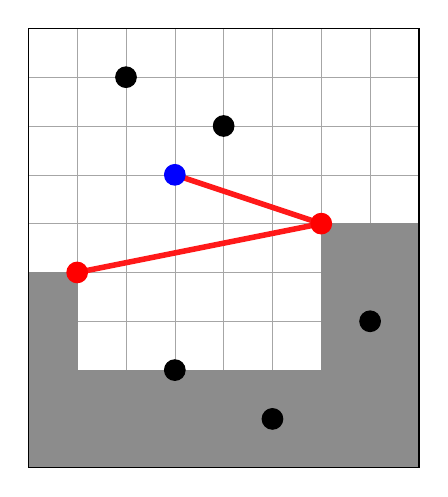
\begin{tikzpicture}[scale=0.62] %4
        \draw[very thin, gray!70] (0,0) grid (8,9);
        
        \draw[fill=gray!90, gray!90] (0,0) rectangle (1,4);
        \draw[fill=gray!90, gray!90] (8,0) rectangle (6,5);
        \draw[fill=gray!90, gray!90] (0,0) rectangle (3,2);
        \draw[fill=gray!90, gray!90] (8,0) rectangle (3,2);

        \draw[red!90, line width=2pt] (3,6) -- (6,5) -- (1,4);

        %\draw[fill=gray!90, gray!90] (10,7) rectangle (11,0);
        %\draw[fill=gray!90, gray!90] (8,6) rectangle (10,0);
        %\draw[fill=gray!90, gray!90] (7,2) rectangle (8,0);    

        \filldraw[black] (5,1) circle (6pt);
        \filldraw[black] (3,2) circle (6pt);
        \filldraw[black] (7,3) circle (6pt);
        \filldraw[red] (1,4) circle (6pt);
        \filldraw[red] (6,5) circle (6pt);
        \filldraw[blue] (3,6) circle (6pt);
        \filldraw[black] (4,7) circle (6pt);
        \filldraw[black] (2,8) circle (6pt);


        %\node at (1,9.5) {\textbf{\Large E}};
        %\node at (2,8.5) {\textbf{\Large E}};
        %\node at (4,5.5) {\textbf{\Large E}};
        %\node at (5,1.5) {\textbf{\Large E}};

        %\node at (10,7.5) {\textbf{\Large D}};
        %\node at (8,6.5) {\textbf{\Large D}};
        %\node at (7,2.5) {\textbf{\Large D}};


        \draw[black, line width=0.5pt] (0,0) rectangle (8,9);
    \end{tikzpicture}
    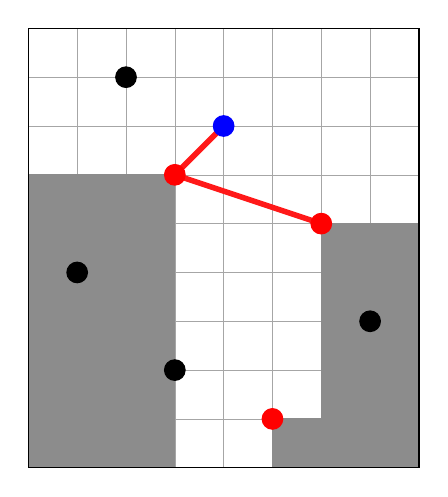
\begin{tikzpicture}[scale=0.62] %5
        \draw[very thin, gray!70] (0,0) grid (8,9);
        
        \draw[fill=gray!90, gray!90] (0,0) rectangle (3,6);
        \draw[fill=gray!90, gray!90] (8,0) rectangle (5,1);
        \draw[fill=gray!90, gray!90] (8,0) rectangle (6,5);
        %\draw[fill=gray!90, gray!90] (1,0) rectangle (2,8);
        %\draw[fill=gray!90, gray!90] (2,0) rectangle (4,5);
        %\draw[fill=gray!90, gray!90] (4,0) rectangle (5,1);

        \draw[red!90, line width=2pt] (4,7) -- (3,6) -- (6,5);
        %\draw[red!90, line width=2pt] (8,6) -- (4,5) -- (7,2) -- (5,1);

        %\draw[fill=gray!90, gray!90] (10,7) rectangle (11,0);
        %\draw[fill=gray!90, gray!90] (8,6) rectangle (10,0);
        %\draw[fill=gray!90, gray!90] (7,2) rectangle (8,0);    

        \filldraw[red] (5,1) circle (6pt);
        \filldraw[black] (3,2) circle (6pt);
        \filldraw[black] (7,3) circle (6pt);
        \filldraw[black] (1,4) circle (6pt);
        \filldraw[red] (6,5) circle (6pt);
        \filldraw[red] (3,6) circle (6pt);
        \filldraw[blue] (4,7) circle (6pt);
        \filldraw[black] (2,8) circle (6pt);


        %\node at (1,9.5) {\textbf{\Large E}};
        %\node at (2,8.5) {\textbf{\Large E}};
        %\node at (4,5.5) {\textbf{\Large E}};
        %\node at (5,1.5) {\textbf{\Large E}};

        %\node at (10,7.5) {\textbf{\Large D}};
        %\node at (8,6.5) {\textbf{\Large D}};
        %\node at (7,2.5) {\textbf{\Large D}};


        \draw[black, line width=0.5pt] (0,0) rectangle (8,9);
    \end{tikzpicture}
    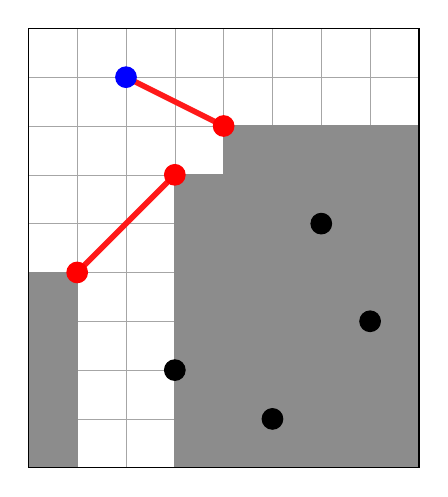
\begin{tikzpicture}[scale=0.62] %6
        \draw[very thin, gray!70] (0,0) grid (8,9);
        
        \draw[fill=gray!90, gray!90] (0,0) rectangle (1,4);
        \draw[fill=gray!90, gray!90] (8,0) rectangle (3,6);
        \draw[fill=gray!90, gray!90] (8,0) rectangle (4,7);

        \draw[red!90, line width=2pt] (2,8) -- (4,7);
        \draw[red!90, line width=2pt] (3,6) -- (1,4);

        \filldraw[black] (5,1) circle (6pt);
        \filldraw[black] (3,2) circle (6pt);
        \filldraw[black] (7,3) circle (6pt);
        \filldraw[red] (1,4) circle (6pt);
        \filldraw[black] (6,5) circle (6pt);
        \filldraw[red] (3,6) circle (6pt);
        \filldraw[red] (4,7) circle (6pt);
        \filldraw[blue] (2,8) circle (6pt);

        \draw[black, line width=0.5pt] (0,0) rectangle (8,9);
    \end{tikzpicture}
\caption{Para a sequência de acessos $X = (5,3,7,1,3,4,2)$, o cálculo de $f(P_X,p)$ para todo $p \in P_X$ é o número de linhas vermelhas. Cada imagem representa o cálculo para o ponto azul, os pontos vermelhos são os pontos pertencentes ao funil do ponto azul e cada linha vermelha representa uma intercalação dos funis esquerdo-direto desse ponto. A imagem dos primeiros dois pontos foi omitida}
\end{figure}
\end{comment}

\begin{figure}
    \centering
    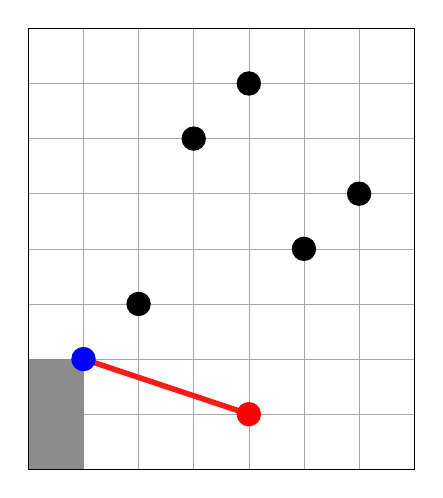
\begin{tikzpicture}[scale=0.7]
        \draw[very thin, gray!70] (0,0) grid (7,8);
        
        \draw[fill=gray!90, gray!90] (0,0) rectangle (1,2);

        \draw[red!90, line width=2pt] (1,2) -- (4,1);  

        \filldraw[red] (4,1) circle (6pt);
        \filldraw[blue] (1,2) circle (6pt);
        \filldraw[black] (2,3) circle (6pt);
        \filldraw[black] (5,4) circle (6pt);
        \filldraw[black] (6,5) circle (6pt);
        \filldraw[black] (3,6) circle (6pt);
        \filldraw[black] (4,7) circle (6pt);


        %\node at (1,9.5) {\textbf{\Large E}};
        %\node at (2,8.5) {\textbf{\Large E}};
        %\node at (4,5.5) {\textbf{\Large E}};
        %\node at (5,1.5) {\textbf{\Large E}};

        %\node at (10,7.5) {\textbf{\Large D}};
        %\node at (8,6.5) {\textbf{\Large D}};
        %\node at (7,2.5) {\textbf{\Large D}};


        \draw[black, line width=0.5pt] (0,0) rectangle (7,8);
    \end{tikzpicture}
    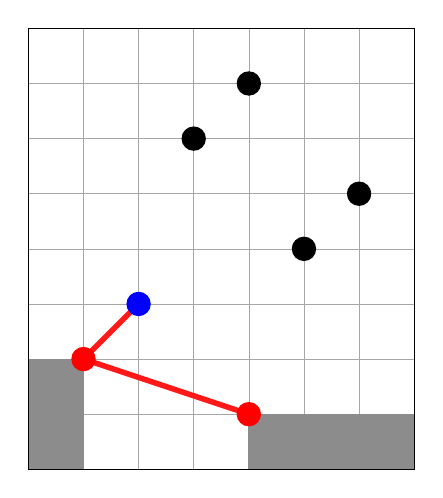
\begin{tikzpicture}[scale=0.7]
        \draw[very thin, gray!70] (0,0) grid (7,8);
        
        \draw[fill=gray!90, gray!90] (0,0) rectangle (1,2);
        \draw[fill=gray!90, gray!90] (7,0) rectangle (4,1);
        %\draw[fill=gray!90, gray!90] (1,0) rectangle (5,1);

        \draw[red!90, line width=2pt] (2,3) -- (1,2) -- (4,1);  

        \filldraw[red] (4,1) circle (6pt);
        \filldraw[red] (1,2) circle (6pt);
        \filldraw[blue] (2,3) circle (6pt);
        \filldraw[black] (5,4) circle (6pt);
        \filldraw[black] (6,5) circle (6pt);
        \filldraw[black] (3,6) circle (6pt);
        \filldraw[black] (4,7) circle (6pt);


        %\node at (1,9.5) {\textbf{\Large E}};
        %\node at (2,8.5) {\textbf{\Large E}};
        %\node at (4,5.5) {\textbf{\Large E}};
        %\node at (5,1.5) {\textbf{\Large E}};

        %\node at (10,7.5) {\textbf{\Large D}};
        %\node at (8,6.5) {\textbf{\Large D}};
        %\node at (7,2.5) {\textbf{\Large D}};


        \draw[black, line width=0.5pt] (0,0) rectangle (7,8);
    \end{tikzpicture}
    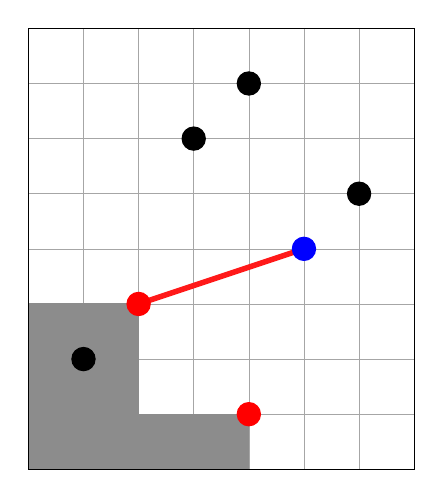
\begin{tikzpicture}[scale=0.7]
        \draw[very thin, gray!70] (0,0) grid (7,8);
        
        \draw[fill=gray!90, gray!90] (0,0) rectangle (4,1);
        \draw[fill=gray!90, gray!90] (0,0) rectangle (2,3);
        %\draw[fill=gray!90, gray!90] (1,0) rectangle (5,1);

        \draw[red!90, line width=2pt] (5,4) -- (2,3);  

        \filldraw[red] (4,1) circle (6pt);
        \filldraw[black] (1,2) circle (6pt);
        \filldraw[red] (2,3) circle (6pt);
        \filldraw[blue] (5,4) circle (6pt);
        \filldraw[black] (6,5) circle (6pt);
        \filldraw[black] (3,6) circle (6pt);
        \filldraw[black] (4,7) circle (6pt);


        %\node at (1,9.5) {\textbf{\Large E}};
        %\node at (2,8.5) {\textbf{\Large E}};
        %\node at (4,5.5) {\textbf{\Large E}};
        %\node at (5,1.5) {\textbf{\Large E}};

        %\node at (10,7.5) {\textbf{\Large D}};
        %\node at (8,6.5) {\textbf{\Large D}};
        %\node at (7,2.5) {\textbf{\Large D}};


        \draw[black, line width=0.5pt] (0,0) rectangle (7,8);
    \end{tikzpicture}
    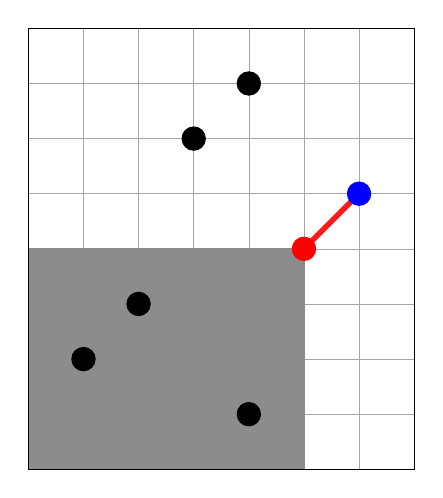
\begin{tikzpicture}[scale=0.7]
        \draw[very thin, gray!70] (0,0) grid (7,8);
        
        \draw[fill=gray!90, gray!90] (0,0) rectangle (5,4);
        %\draw[fill=gray!90, gray!90] (1,0) rectangle (5,1);

        \draw[red!90, line width=2pt] (6,5) -- (5,4);  

        \filldraw[black] (4,1) circle (6pt);
        \filldraw[black] (2,3) circle (6pt);
        \filldraw[black] (1,2) circle (6pt);
        \filldraw[red] (5,4) circle (6pt);
        \filldraw[blue] (6,5) circle (6pt);
        \filldraw[black] (3,6) circle (6pt);
        \filldraw[black] (4,7) circle (6pt);


        %\node at (1,9.5) {\textbf{\Large E}};
        %\node at (2,8.5) {\textbf{\Large E}};
        %\node at (4,5.5) {\textbf{\Large E}};
        %\node at (5,1.5) {\textbf{\Large E}};

        %\node at (10,7.5) {\textbf{\Large D}};
        %\node at (8,6.5) {\textbf{\Large D}};
        %\node at (7,2.5) {\textbf{\Large D}};


        \draw[black, line width=0.5pt] (0,0) rectangle (7,8);
    \end{tikzpicture}
    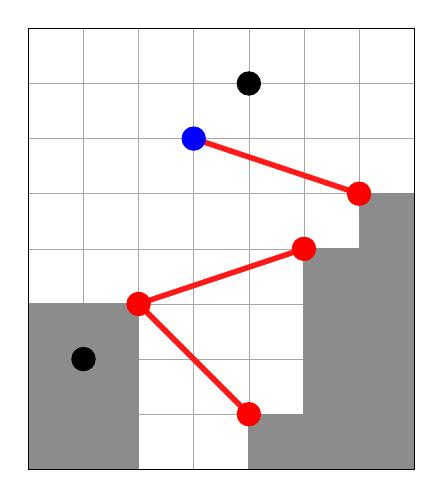
\begin{tikzpicture}[scale=0.7]
        \draw[very thin, gray!70] (0,0) grid (7,8);
        
        \draw[fill=gray!90, gray!90] (7,0) rectangle (6,5);
        \draw[fill=gray!90, gray!90] (7,0) rectangle (5,4);
        \draw[fill=gray!90, gray!90] (0,0) rectangle (2,3);
        \draw[fill=gray!90, gray!90] (7,0) rectangle (4,1);
        %\draw[fill=gray!90, gray!90] (1,0) rectangle (5,1);

        \draw[red!90, line width=2pt] (3,6) -- (6,5);  
        \draw[red!90, line width=2pt] (5,4) -- (2,3) -- (4,1);  

        \filldraw[red] (4,1) circle (6pt);
        \filldraw[red] (2,3) circle (6pt);
        \filldraw[black] (1,2) circle (6pt);
        \filldraw[red] (5,4) circle (6pt);
        \filldraw[red] (6,5) circle (6pt);
        \filldraw[blue] (3,6) circle (6pt);
        \filldraw[black] (4,7) circle (6pt);


        %\node at (1,9.5) {\textbf{\Large E}};
        %\node at (2,8.5) {\textbf{\Large E}};
        %\node at (4,5.5) {\textbf{\Large E}};
        %\node at (5,1.5) {\textbf{\Large E}};

        %\node at (10,7.5) {\textbf{\Large D}};
        %\node at (8,6.5) {\textbf{\Large D}};
        %\node at (7,2.5) {\textbf{\Large D}};


        \draw[black, line width=0.5pt] (0,0) rectangle (7,8);
    \end{tikzpicture}
    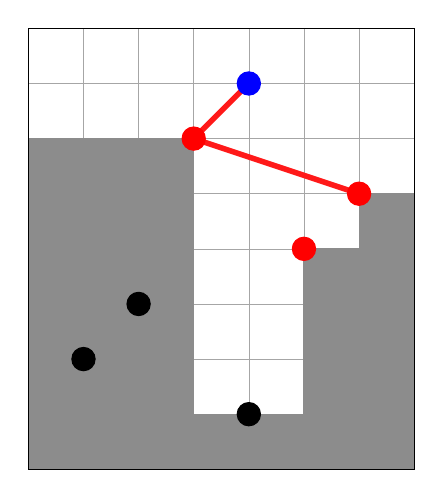
\begin{tikzpicture}[scale=0.7]
        \draw[very thin, gray!70] (0,0) grid (7,8);
        
        \draw[fill=gray!90, gray!90] (0,0) rectangle (3,6);
        \draw[fill=gray!90, gray!90] (7,0) rectangle (6,5);
        \draw[fill=gray!90, gray!90] (7,0) rectangle (5,4);
        \draw[fill=gray!90, gray!90] (0,0) rectangle (4,1);
        \draw[fill=gray!90, gray!90] (7,0) rectangle (4,1);

        \draw[red!90, line width=2pt] (4,7) -- (3,6) -- (6,5);  

        \filldraw[black] (4,1) circle (6pt);
        \filldraw[black] (2,3) circle (6pt);
        \filldraw[black] (1,2) circle (6pt);
        \filldraw[red] (5,4) circle (6pt);
        \filldraw[red] (6,5) circle (6pt);
        \filldraw[red] (3,6) circle (6pt);
        \filldraw[blue] (4,7) circle (6pt);


        %\node at (1,9.5) {\textbf{\Large E}};
        %\node at (2,8.5) {\textbf{\Large E}};
        %\node at (4,5.5) {\textbf{\Large E}};
        %\node at (5,1.5) {\textbf{\Large E}};

        %\node at (10,7.5) {\textbf{\Large D}};
        %\node at (8,6.5) {\textbf{\Large D}};
        %\node at (7,2.5) {\textbf{\Large D}};


        \draw[black, line width=0.5pt] (0,0) rectangle (7,8);
    \end{tikzpicture}    
\caption{Para a sequência de acessos $X = (4,1,2,5,6,3,4)$, o cálculo de $f(P_X,p)$ para todo $p \in P_X$ é o número de linhas vermelhas. Cada imagem representa o cálculo de $f(P_X,p)$ para o ponto azul $p$, os pontos vermelhos são os pontos pertencentes ao funil de $p$ e cada linha vermelha representa uma intercalação dos funis esquerdo-direto desse ponto. Para essa sequência de acessos, Funil$(X) = 9$.}
\end{figure}

\section{Conjunto independente de retângulos no funil}

Por definição, todos os pontos $q$ do funil de um ponto $p$ possuem a propriedade que o $\{p,q\}$-retângulo está arboreamente insatisfeito.